\RequirePackage[OT1]{fontenc} 
\documentclass[journal]{IEEEtran}

% *** CITATION PACKAGES ***
\usepackage[style=ieee]{biblatex} 
\bibliography{example_bib.bib}    %your file created using JabRef

% *** MATH PACKAGES ***
\usepackage{amsmath}

% Table Packages
\usepackage{booktabs}
\usepackage{tabularx}

% *** PDF, URL AND HYPERLINK PACKAGES ***
\usepackage{url}
% correct bad hyphenation here
\hyphenation{op-tical net-works semi-conduc-tor}
\usepackage{graphicx}  %needed to include png, eps figures
\graphicspath{{./images/}}
\usepackage{float}  % used to fix location of images i.e.\begin{figure}[H]

\begin{document}

% paper title
\newcommand{\LabNumber}{\#5}
\newcommand{\LabTitle}{Half-Wave Dipole Antenna}

\title{RF Lab Module \LabNumber\ --- \LabTitle}
%\\ \small{Title of the session (you can be creative highlighting your findings)}}

% author names 
\author{Stephen Campbell
    % Student 2 First Name Last Name 
}% <-this % stops a space

% The report headers
\markboth{EE/CE 4202 Electrical and Computer Engineering Laboratory in Circuits. Lab \LabNumber, \today}%do not delete next lines
{Shell \MakeLowercase{\textit{et al.}}: Bare Demo of IEEEtran.cls for IEEE Journals}

% make the title area
\maketitle

% As a general rule, do not put math, special symbols or citations
% in the abstract or keywords.
\begin{abstract}
    This lab focuses on the design and analysis of a half wave dipole antenna and
    how using it affects the magnitude of the radio frequency signal received from a
    cell phone. Two antennas were manufactured to have their resonant frequency at
    our test cell phone's de facto frequency. Different configurations were measured
    and analyzed including using no antenna and cellphone, cell phone to antenna,
    and antenna to antenna. Each configuration elucidated the clear need for
    antenna's in todays wireless world.
\end{abstract}

\section{Introduction}

\IEEEPARstart{T}{he} modern cellphone is capable of communication at a variety
of frequency bands. This lab considers simply the one most easily measurable in
practice, in our case 1.8 GHz. With the frequency in mind, our half wave dipole
antenna was custom made to best receive the cell phone's signal. The half wave
dipole antenna is a straightforward antenna design that, for our purposes only
requires a SMA connector and wire. By having 2 antennas manufactured, our
procedure allowed for a transmit antenna to be compared with the cell phone's
antenna with both having their power received from the same receive antenna. The
procedure explores how antennas' distance, orientation, and size play into their
effectiveness.

\section{Procedure}
\begin{enumerate}
    \item Determine cell phone's operating frequency without an antenna
          \begin{enumerate}
              \item Connect a coax line to the spectrum analyzer
              \item Move the cable in proximity to the test cell phone
              \item Make a call and note the frequency with the largest power response
          \end{enumerate}
    \item Construct a half wave dipole antenna with the resonant frequency of the operating frequency
          \begin{enumerate}
              \item Using the operating frequency, determine the quarter wave length
              \item Cut 2 wire strip a quarter wave length
              \item Solder each wire strip to a SMA connector
              \item Measure the S11 and note the dip as the resonant frequency
          \end{enumerate}
    \item Measure the received power from the cell phone using the antenna
          \begin{enumerate}
              \item Connect the antenna to the spectrum analyzer
              \item Make a call and note the signal strength at the operating frequency
          \end{enumerate}
    \item Construct an identical antenna as in step 2 (Repeat step 2)
    \item Measure the received power of the antenna
          \begin{enumerate}
              \item Connect an antenna to the signal generator as the transmitting antenna. Output 0dB at the cell phone operating frequency
              \item Connect an antenna to the spectrum analyzer as the receiving antenna
              \item With both antenna's in the same orientation measure the received power if they are 30,20,10 cm away.
              \item With their orientations 90 degrees out of phase Measure the received power at 20 cm away.
          \end{enumerate}
    \item Measure the received power of the cell phone
          \begin{enumerate}
              \item Connect an antenna to the spectrum analyzer as the receiving antenna
              \item Make a call  and measure the received power if the cell phone and antenna are 30,20,10 cm apart.
          \end{enumerate}
\end{enumerate}

\section{Analysis}
Our test cell phone was measured to have an operating frequency of 1.8GHz with
an absolute power of -20dBm without an antenna. The power measured when calling
with the cellphone was -10dBm with the antenna. Thus, the absolute power was 10
dB larger with the antenna.

\textbf{ Record your measurements and create a table of data.}
The tables of data are located at Table~\ref{table:freq} and Table~\ref{table:power}.

\begin{figure}[hp]
    \centering
    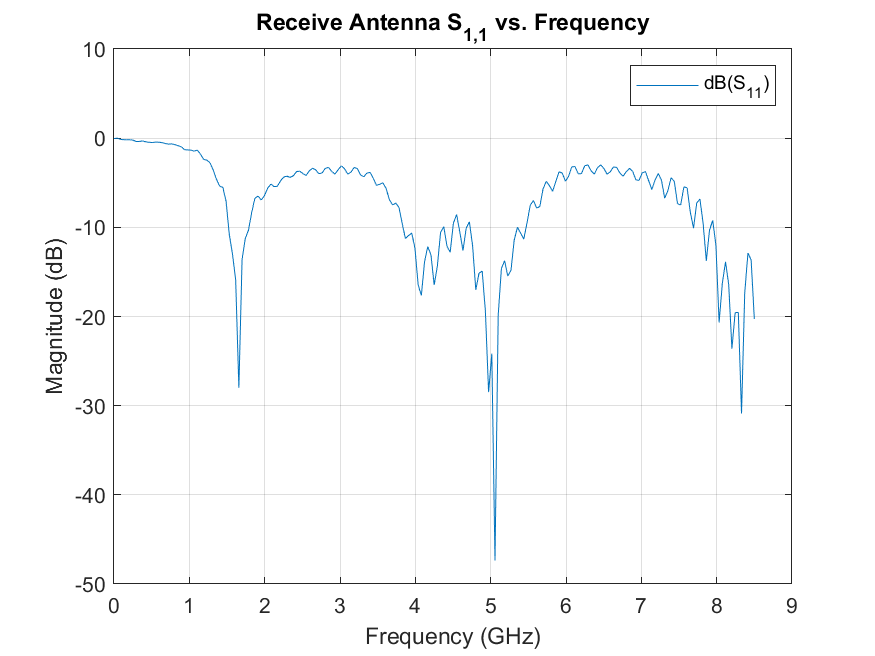
\includegraphics[width=0.3\textwidth]{receive_rl.png}

    \caption{\label{fig:recv} \(S_{1,1}\) vs. Frequency of Receive Antenna}
\end{figure}

\begin{figure}[hp]
    \centering
    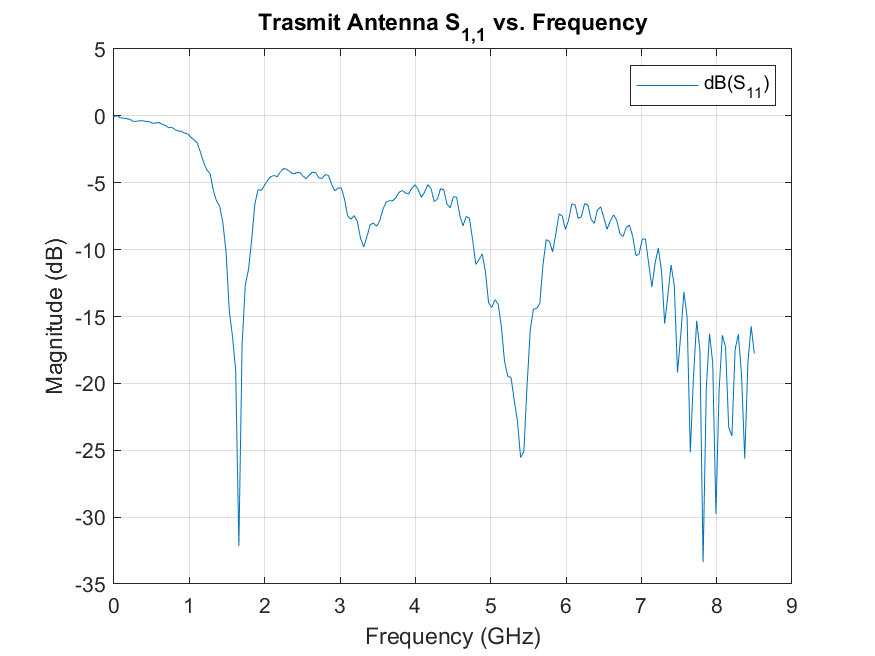
\includegraphics[width=0.3\textwidth]{transmit_rl.png}

    \caption{\label{fig:transmit} \(S_{1,1}\) vs. Frequency of Transmit Antenna}
\end{figure}


\begin{table}[hp]
    \centering
    \begin{tabular}{|l|l|}
        \toprule
        Antenna  & Resonant Frequency (GHz) \\ \midrule
        Transmit & 1.6                      \\ \midrule
        Receive  & 1.8                      \\ \bottomrule
    \end{tabular}
    \vspace{1em}
    \caption{\label{table:freq} Resonant Frequencies of Constructed Antennas}
\end{table}

\begin{table}[hp]
    \centering
    \begin{tabular}{ll}
        \toprule
        \multicolumn{1}{|l|}{Distance (cm)} & \multicolumn{1}{l|}{Measured Power (dBm)} \\ \midrule
        \multicolumn{2}{|l|}{\textbf{Antenna to Antenna (Same Orientation)}}            \\ \midrule
        \multicolumn{1}{|l|}{30}            & \multicolumn{1}{l|}{-35}                  \\ \midrule
        \multicolumn{1}{|l|}{20}            & \multicolumn{1}{l|}{-23}                  \\ \midrule
        \multicolumn{1}{|l|}{10}            & \multicolumn{1}{l|}{-18}                  \\ \midrule
        \multicolumn{2}{|l|}{\textbf{Antenna to Antenna (Perpendicular Orientation)}}   \\ \midrule
        \multicolumn{1}{|l|}{20}            & \multicolumn{1}{l|}{-40}                  \\ \midrule
        \multicolumn{2}{|l|}{\textbf{Cell Phone to Antenna}}                            \\ \midrule
        \multicolumn{1}{|l|}{30}            & \multicolumn{1}{l|}{-42}                  \\ \midrule
        \multicolumn{1}{|l|}{20}            & \multicolumn{1}{l|}{-38}                  \\ \midrule
        \multicolumn{1}{|l|}{10}            & \multicolumn{1}{l|}{-15}                  \\ \bottomrule
    \end{tabular}

    \vspace{1em}
    \caption{\label{table:power} Measured powers across configurations}
\end{table}

\textbf{ From the measurements you made, estimate the transmitted power (in dBm) of your cell phone.}
With the possibly poor assumption that the cell phone antenna will have a
similar transmit/receive ratio as the half-dipole antenna to antenna
configuration. It is estimated that the cell phone is transmitting 0dBm or 1 mW
of power.

\textbf{ What was your measured cross-polarization isolation? Why is it important to keep antennas aligned with the proper polarization?}

When the signal generator was transmitting 0dBm through the transmit antenna the
receive antenna at the 90 degree orientation received -40dBm.  The
cross-polarization isolation at 20cm is -40dB. It is important to keep antennas
aligned with the proper polarization because misalignment can mean extremely
significant losses and a very poor signal to noise ratio.


\textbf{ Include photos of your antennas and measurement set-ups (cell phone transmit power measurement, etc.)}

\begin{figure}[hp]
    \centering
    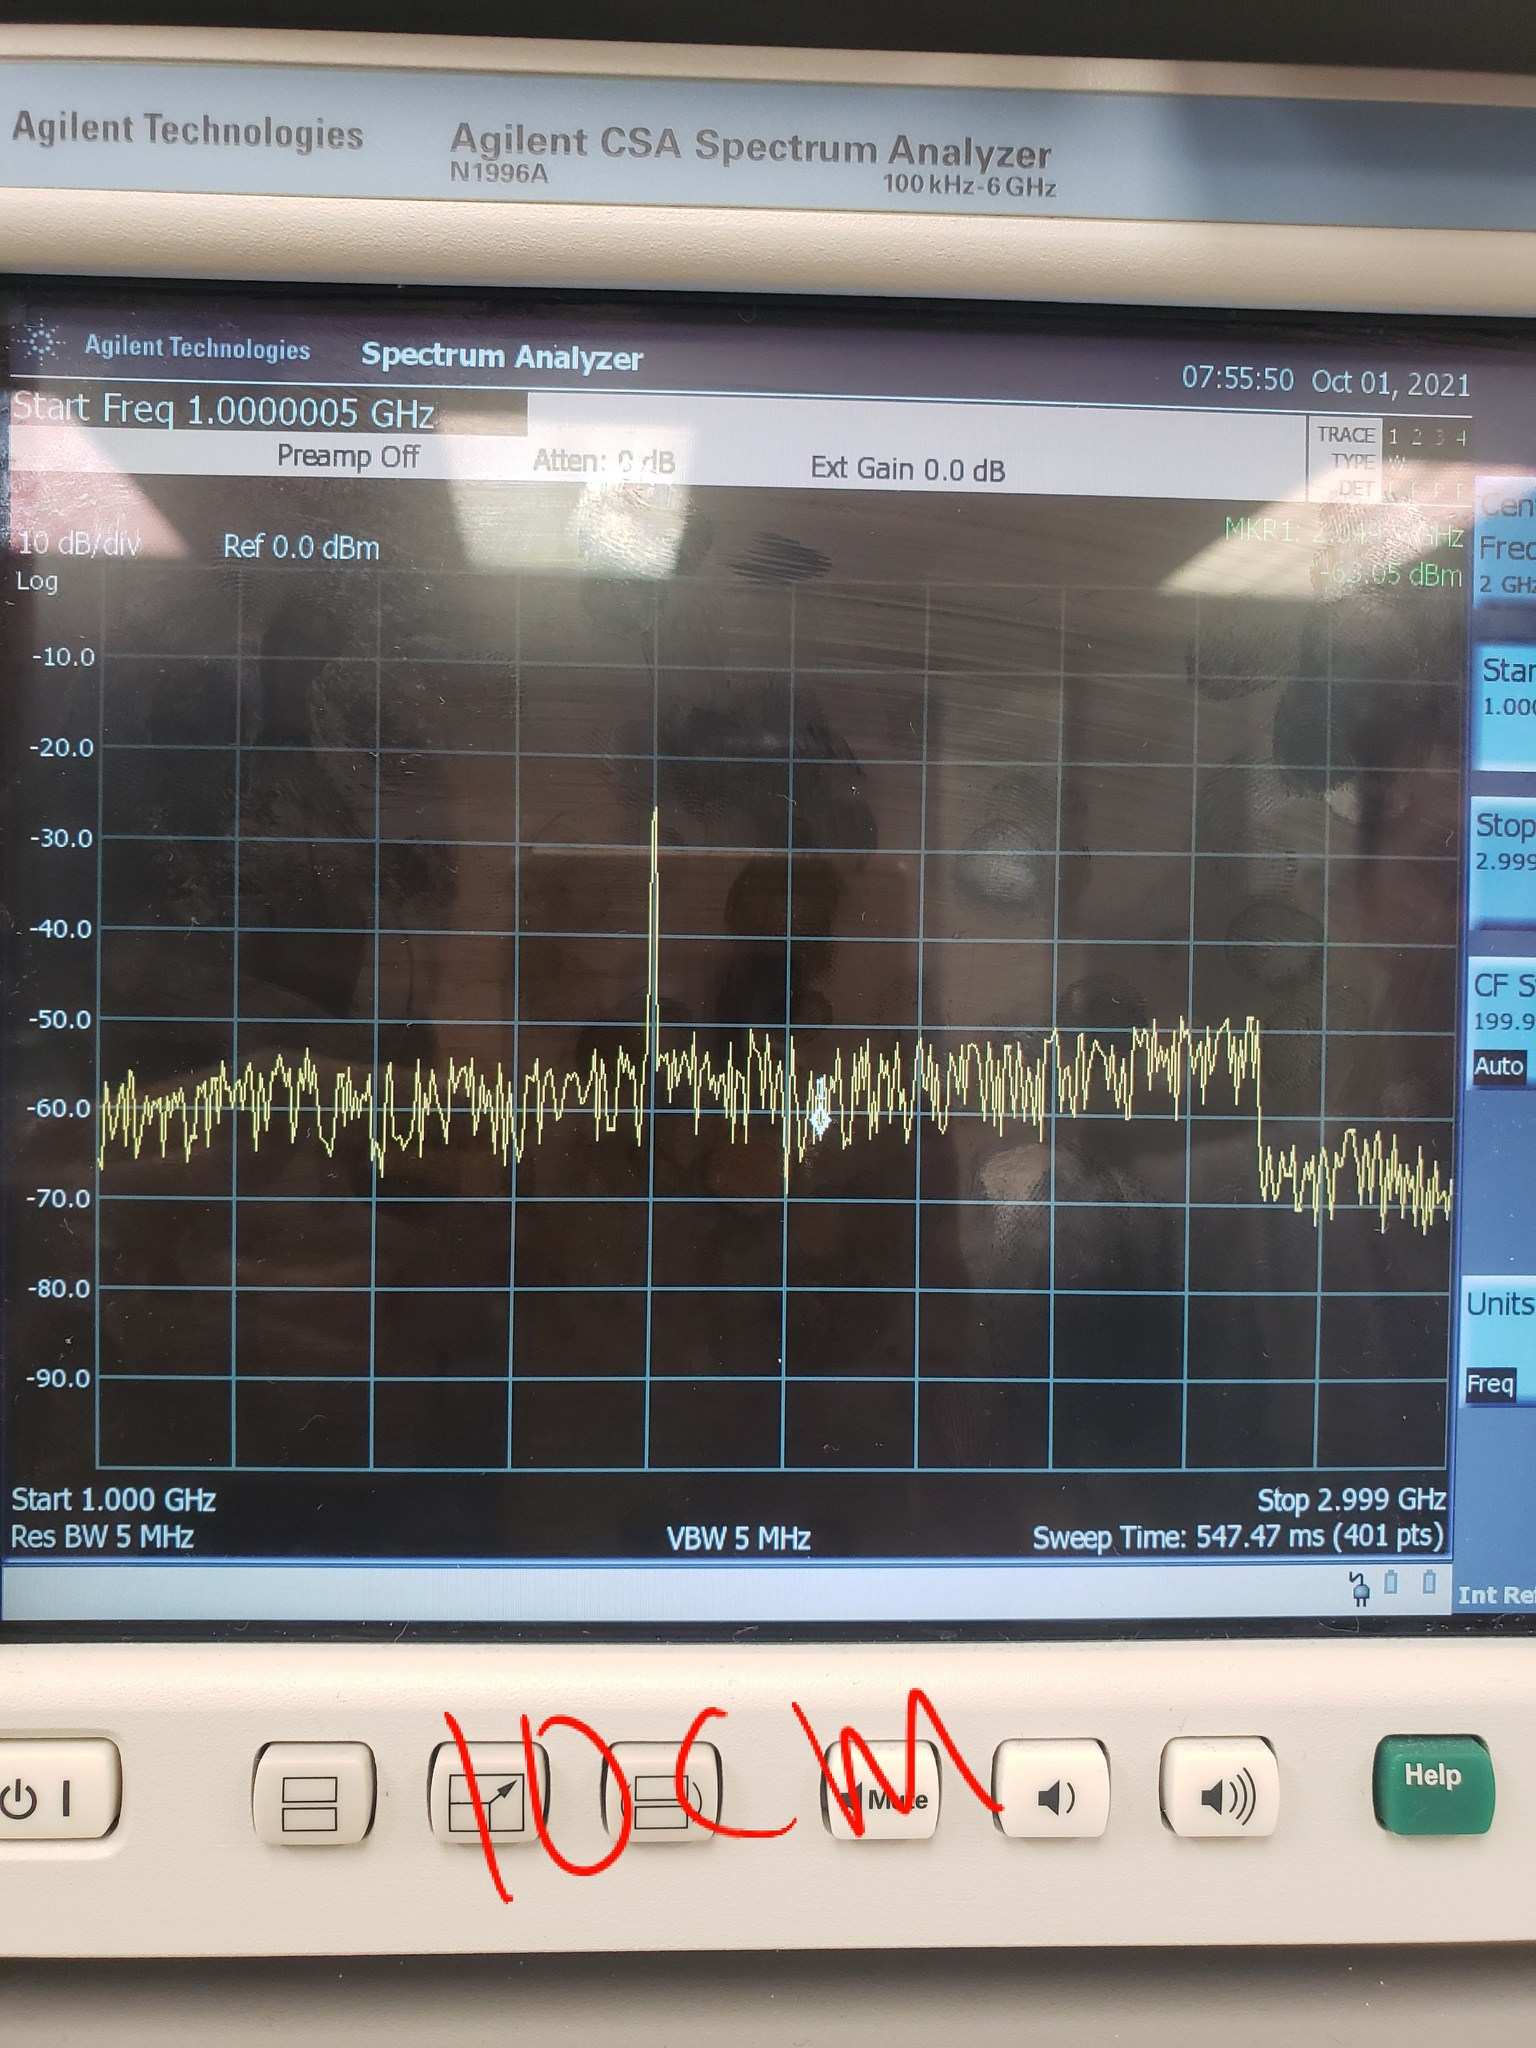
\includegraphics[width=0.3\textwidth]{txrx_10.JPG}
    \caption{\label{fig:txrx_10} Antenna to Antenna Power Measurement from 10cm apart}
\end{figure}

\begin{figure}[hp]
    \centering
    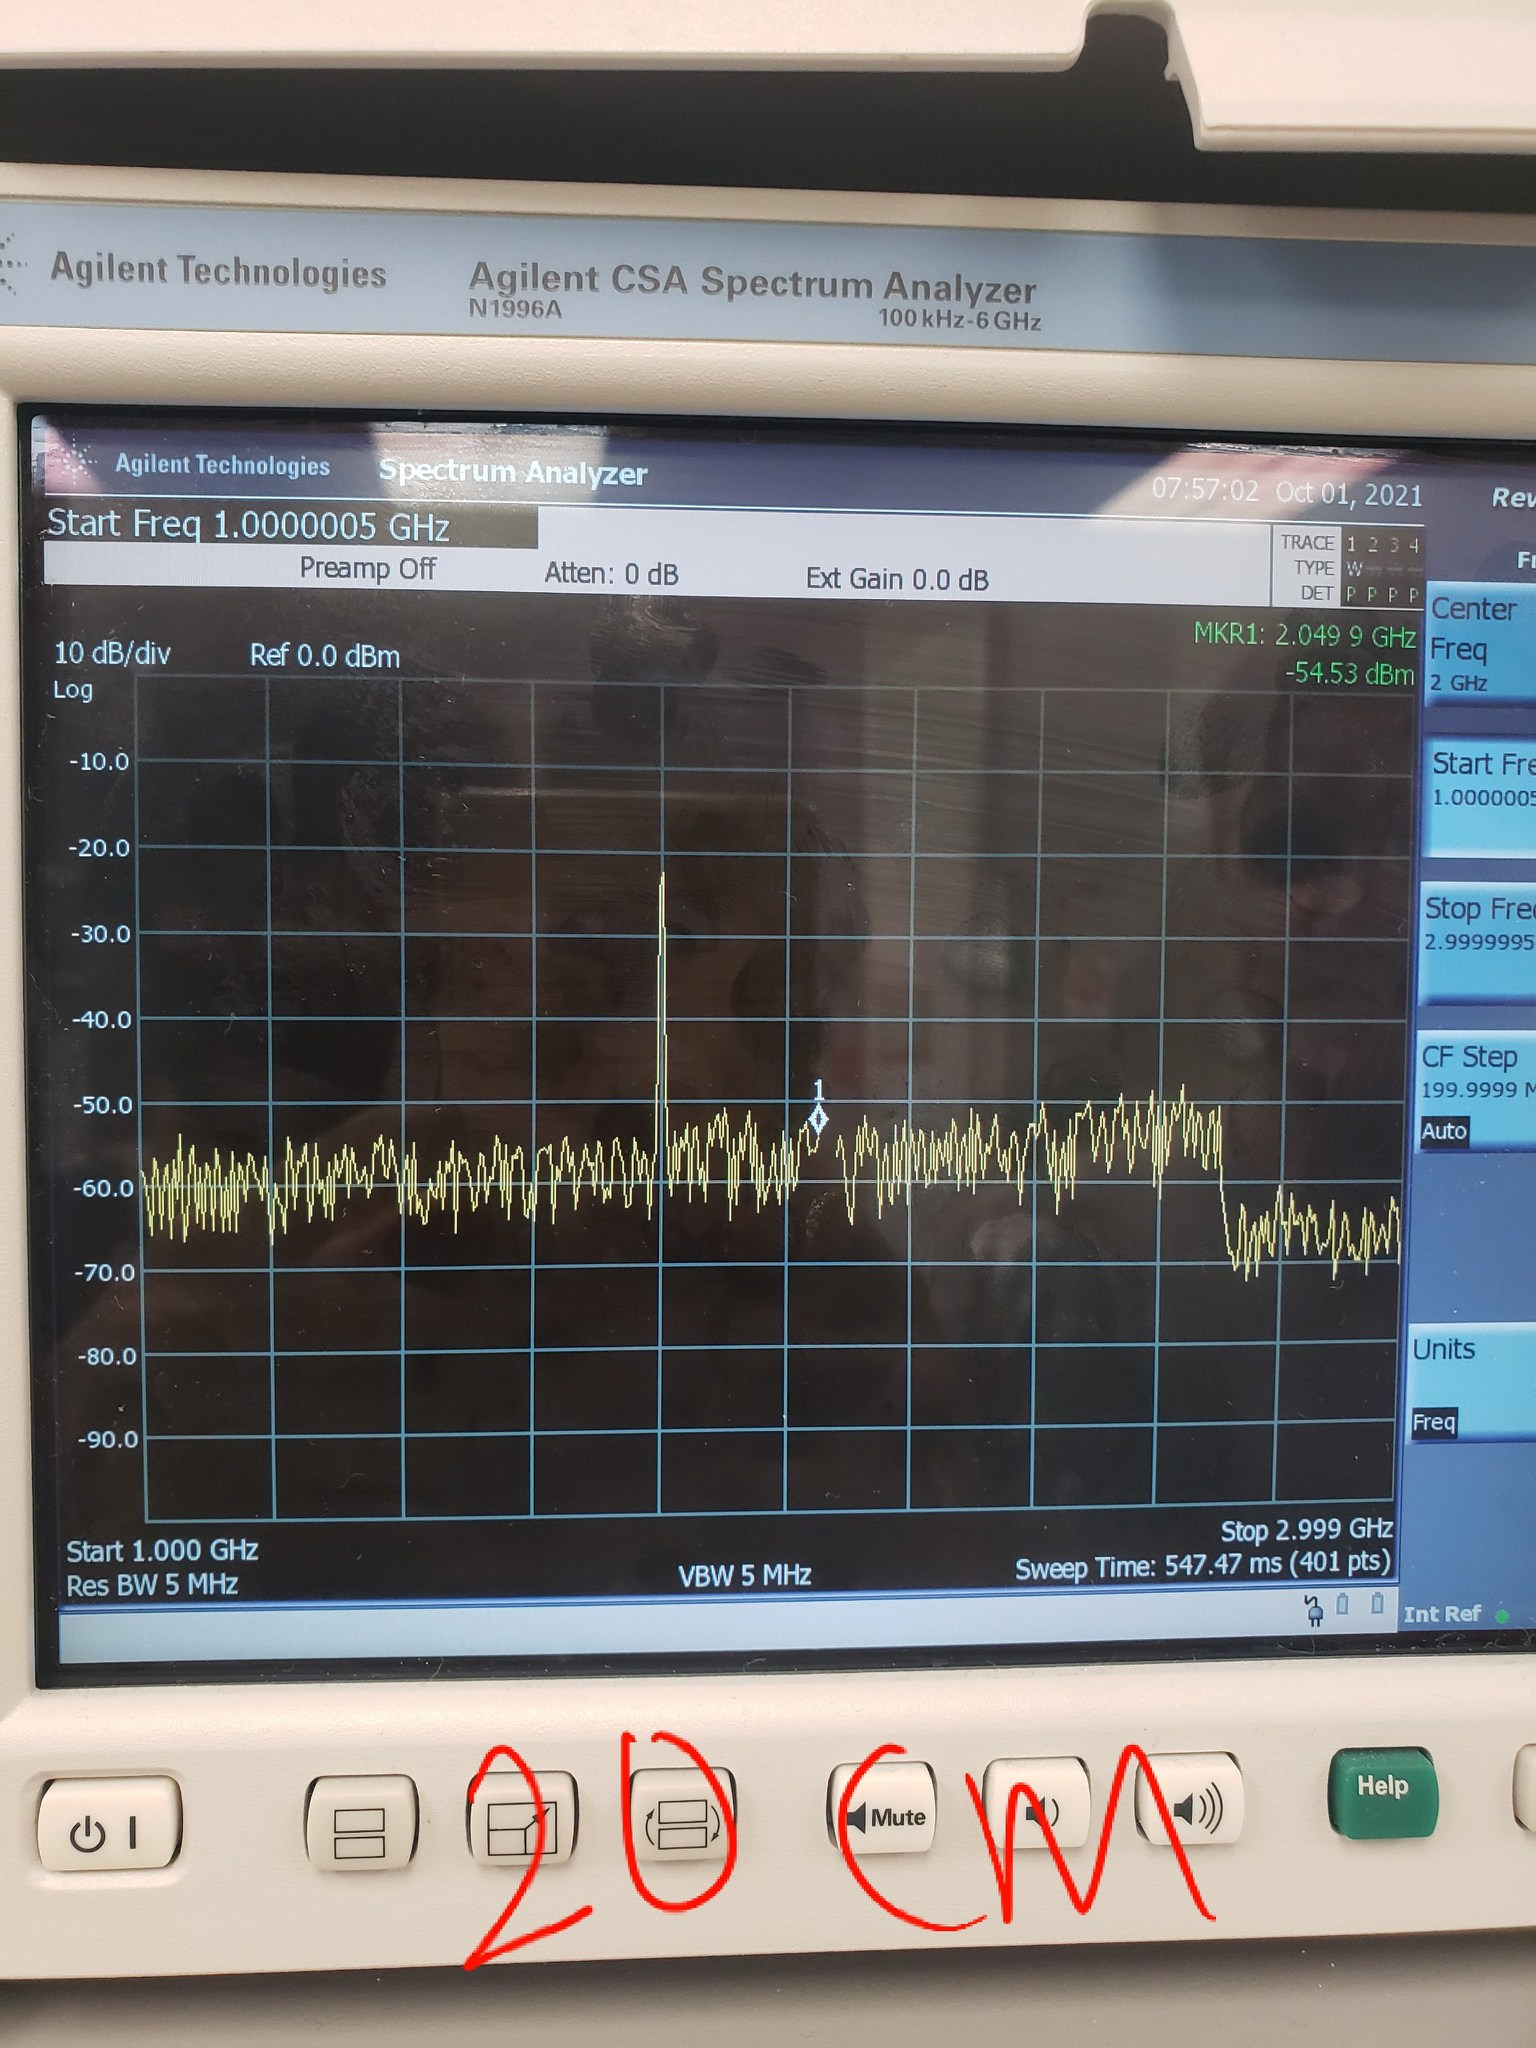
\includegraphics[width=0.3\textwidth]{txrx_20.JPG}
    \caption{\label{fig:txrx_20} Antenna to Antenna Power Measurement from 20cm apart}
\end{figure}

\begin{figure}[hp]
    \centering
    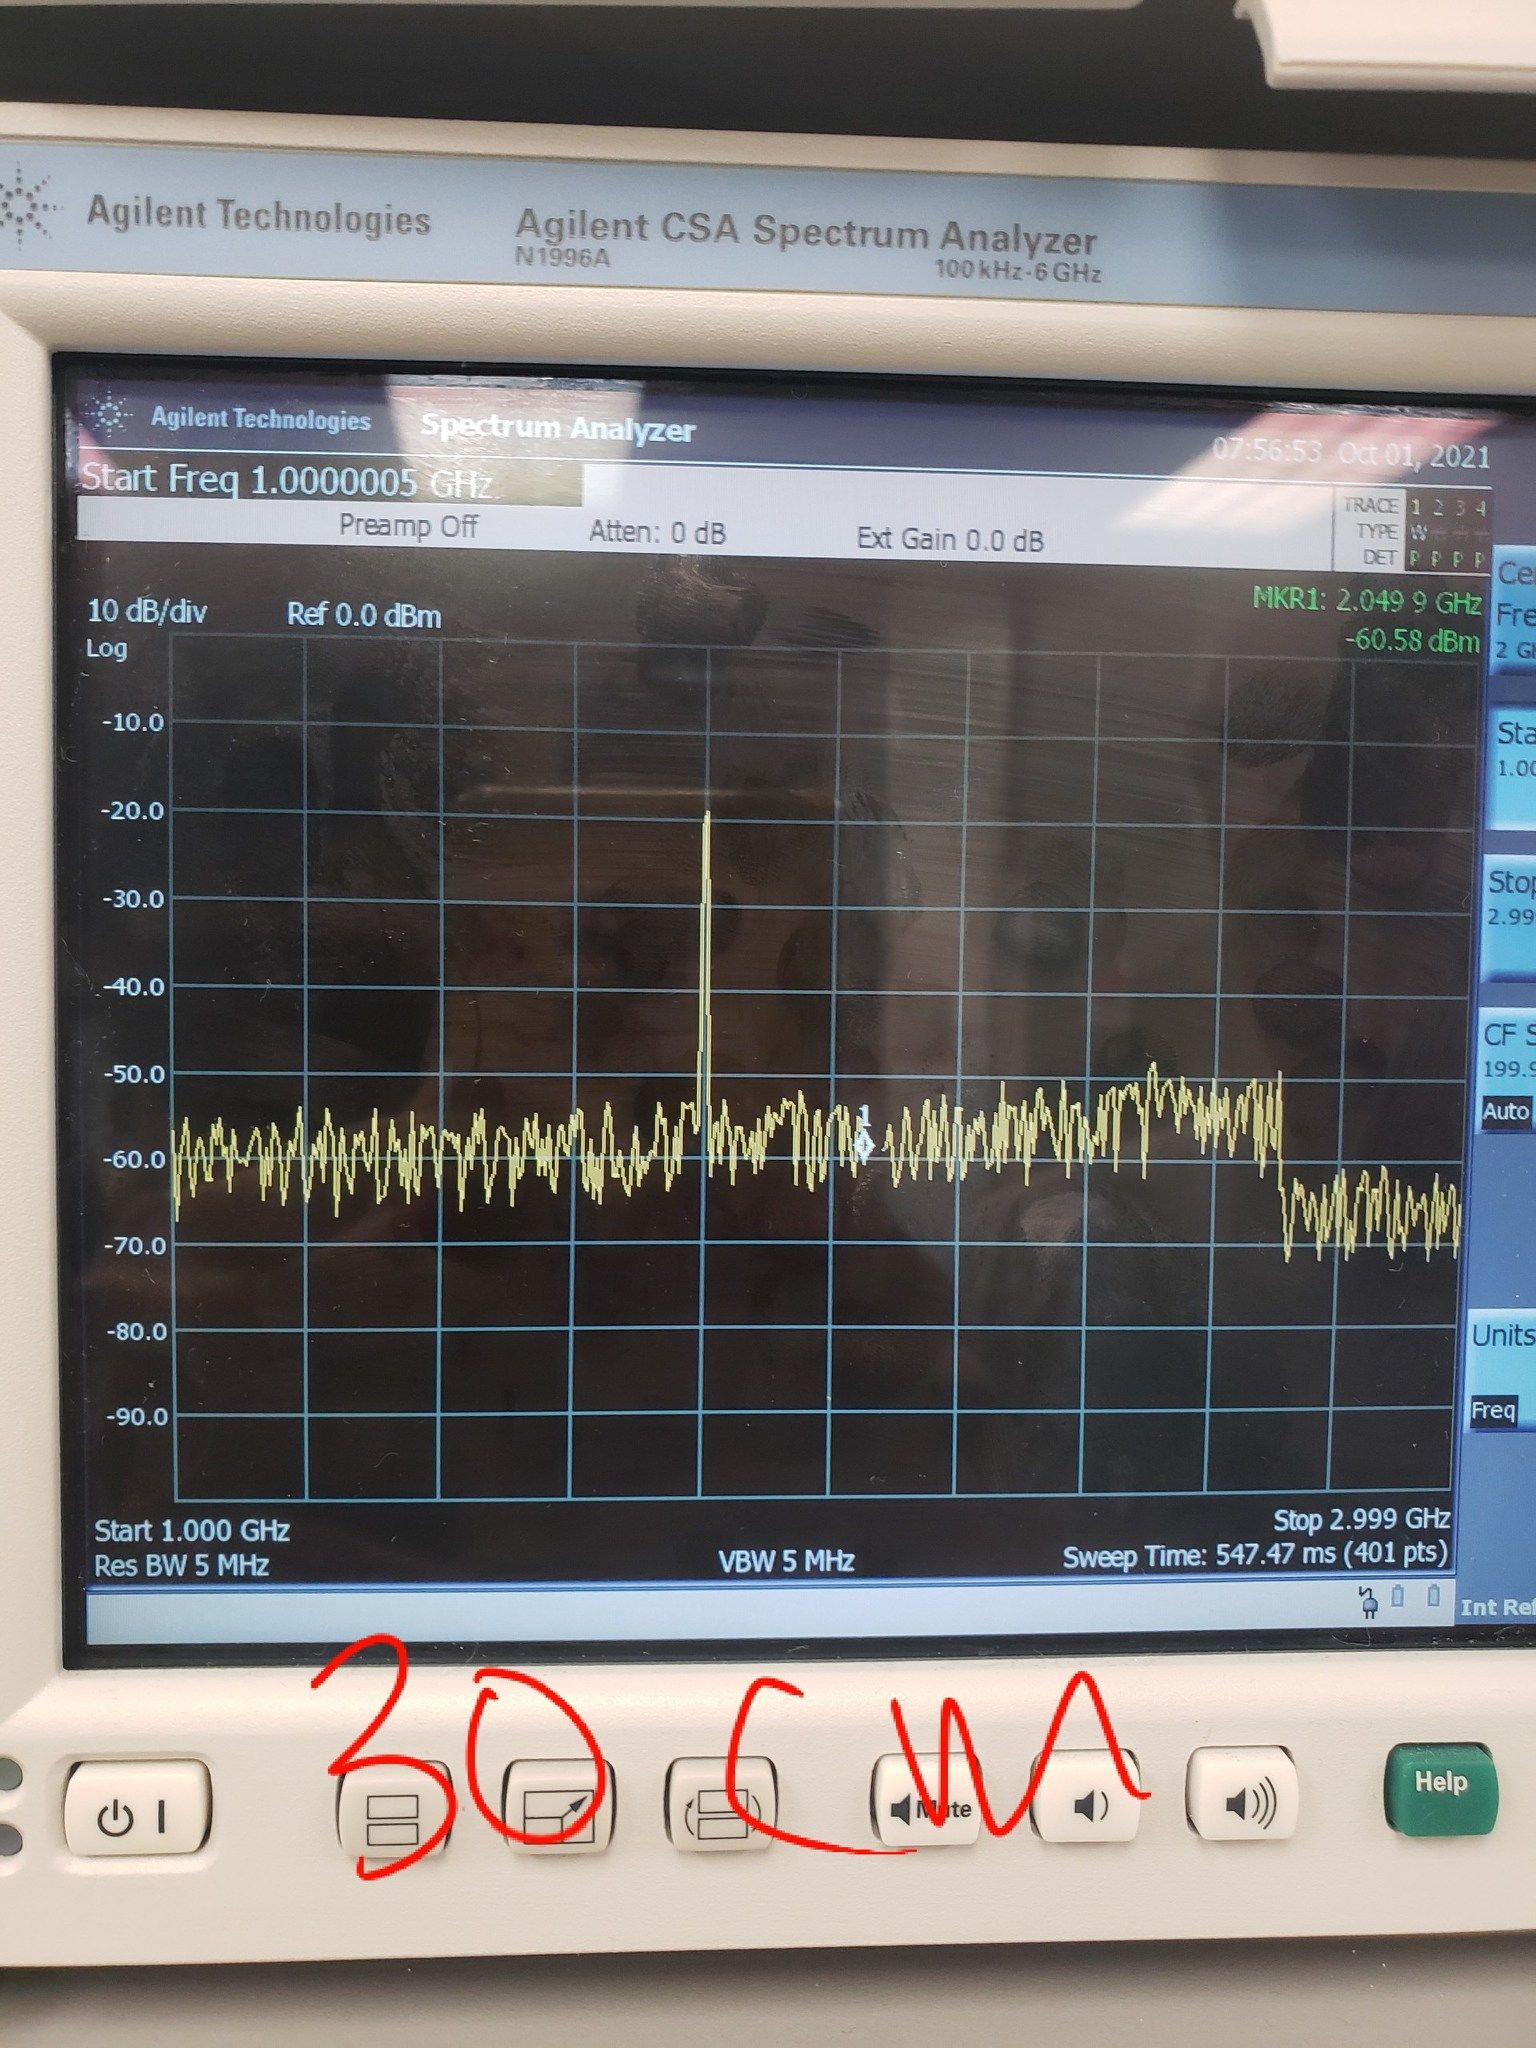
\includegraphics[width=0.3\textwidth]{txrx_30.JPG}
    \caption{\label{fig:txrx_30} Antenna to Antenna Power Measurement from 30cm apart}
\end{figure}

\begin{figure}[hp]
    \centering
    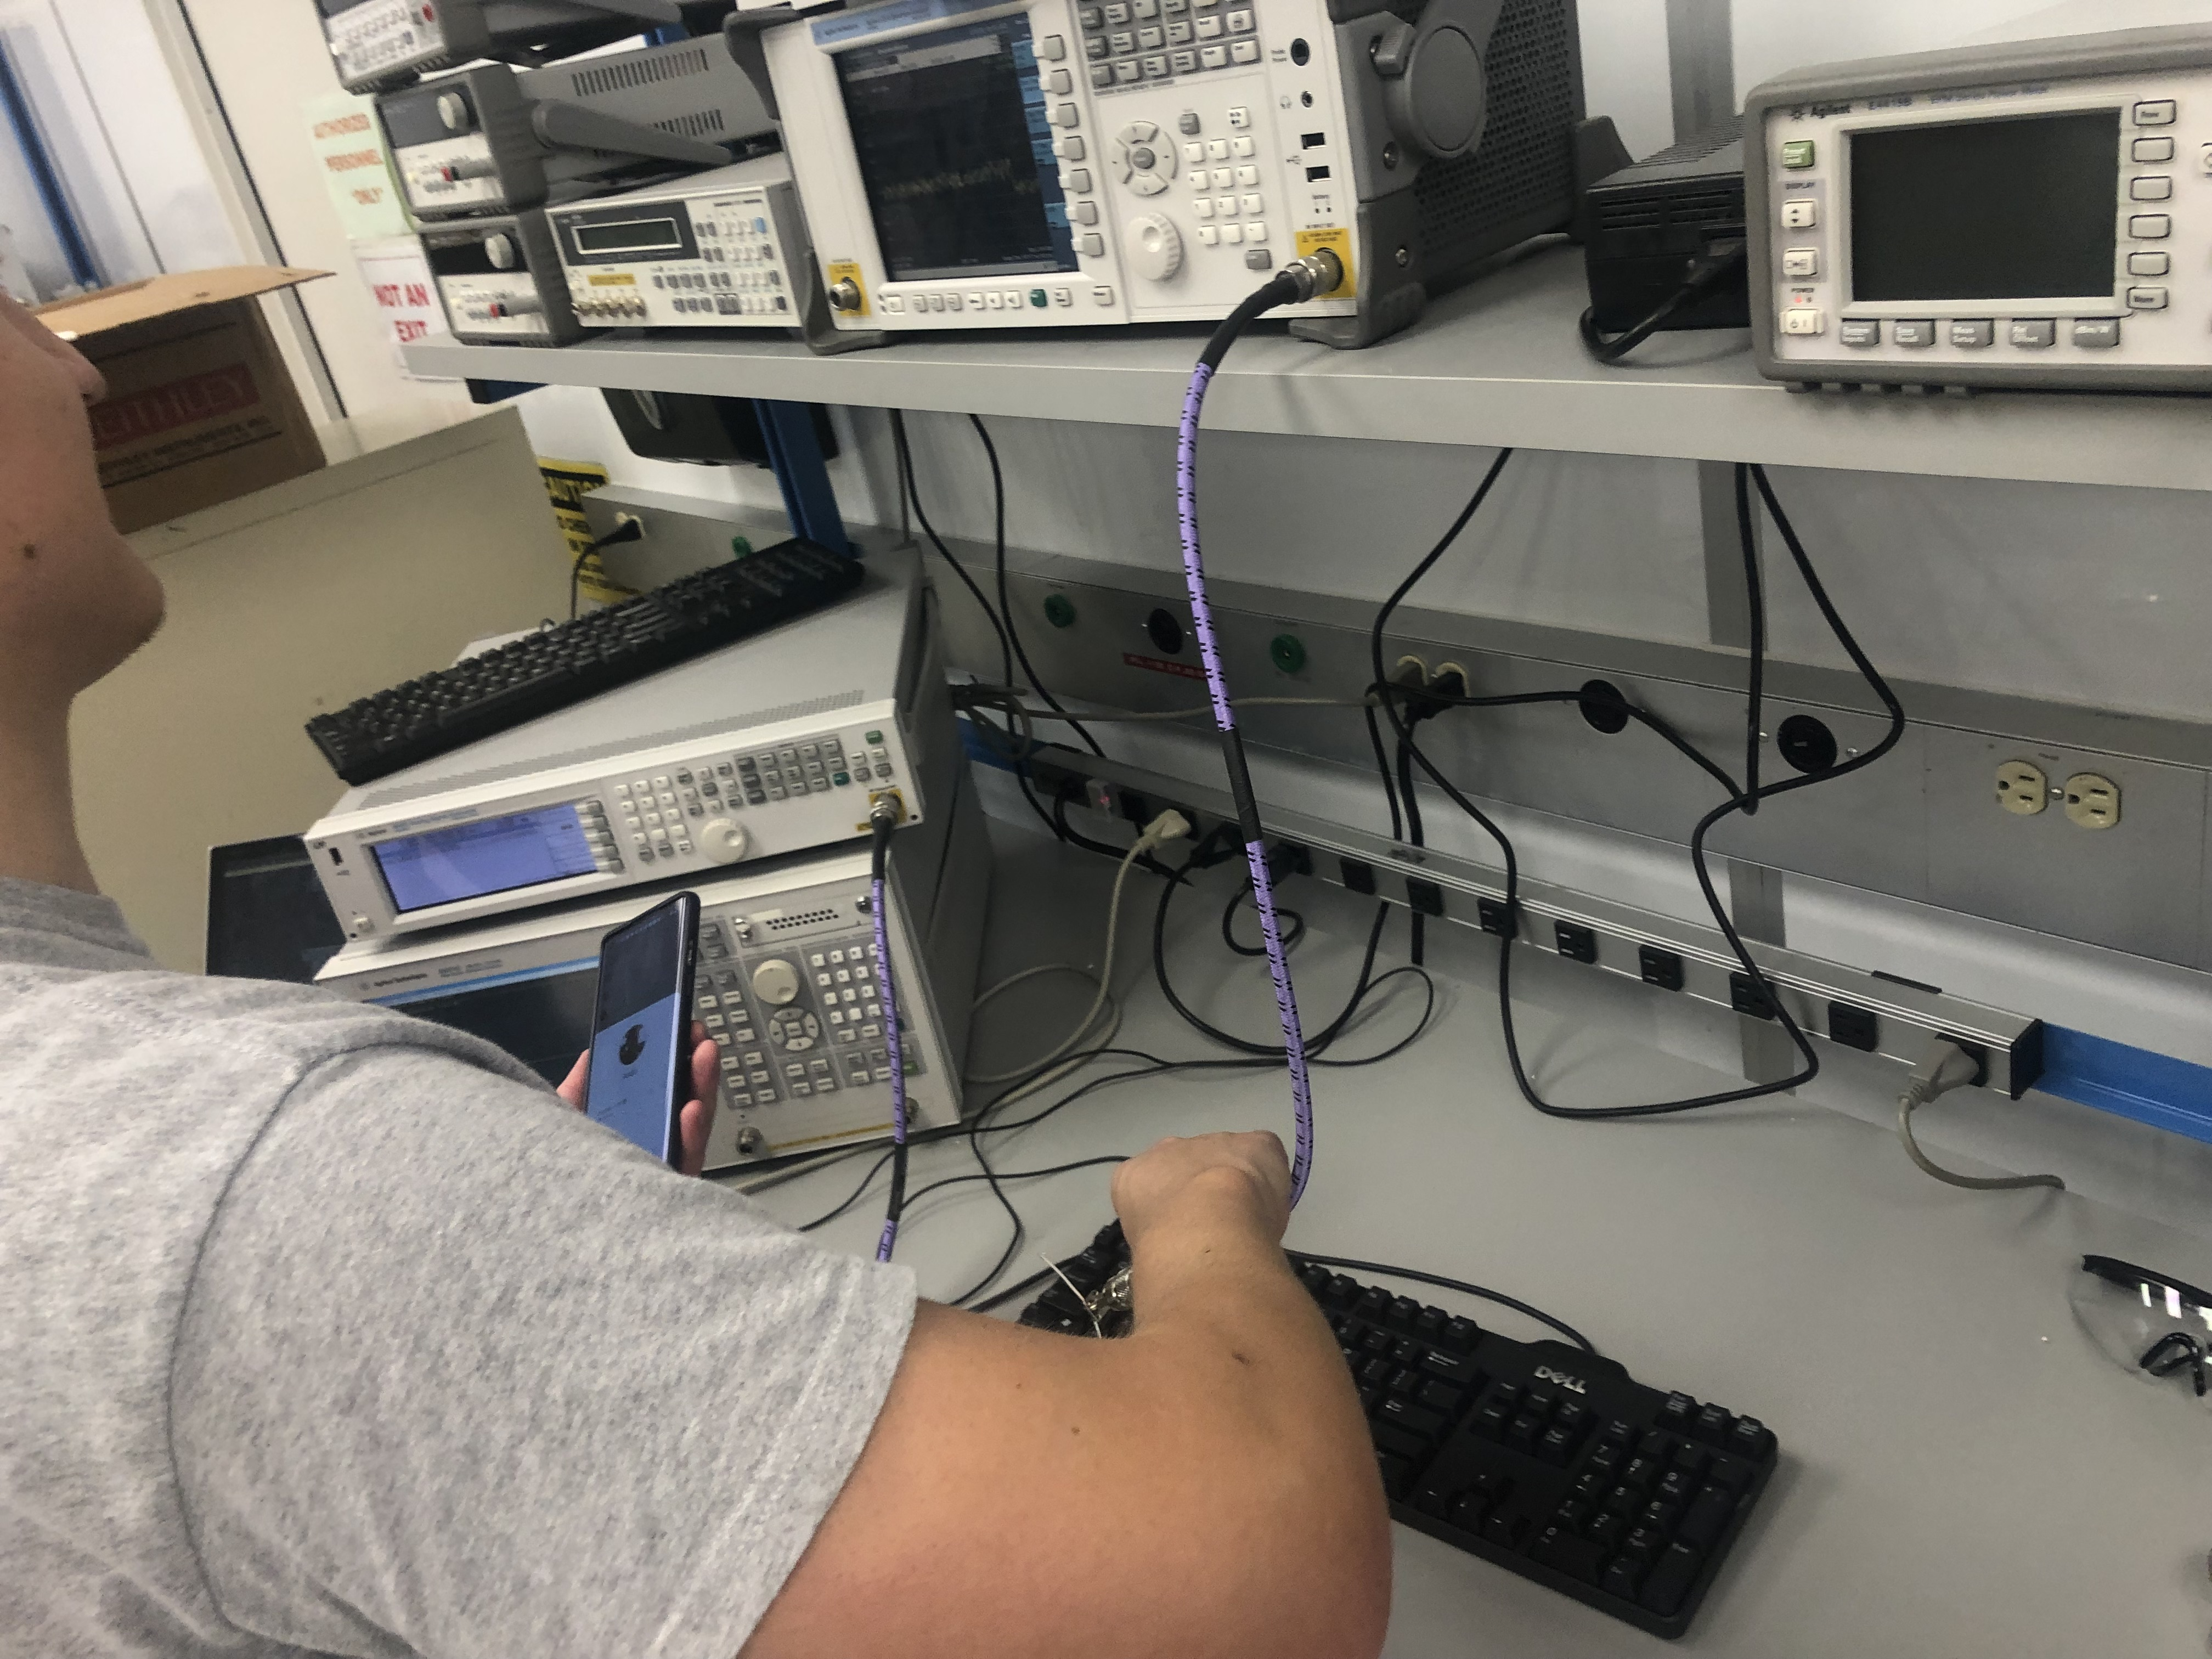
\includegraphics[width=0.3\textwidth]{phonerx_setup.jpg}
    \caption{\label{fig:phonerx_setup} Phone to Antenna Power Measurement Setup}
\end{figure}

\begin{figure}[hp]
    \centering
    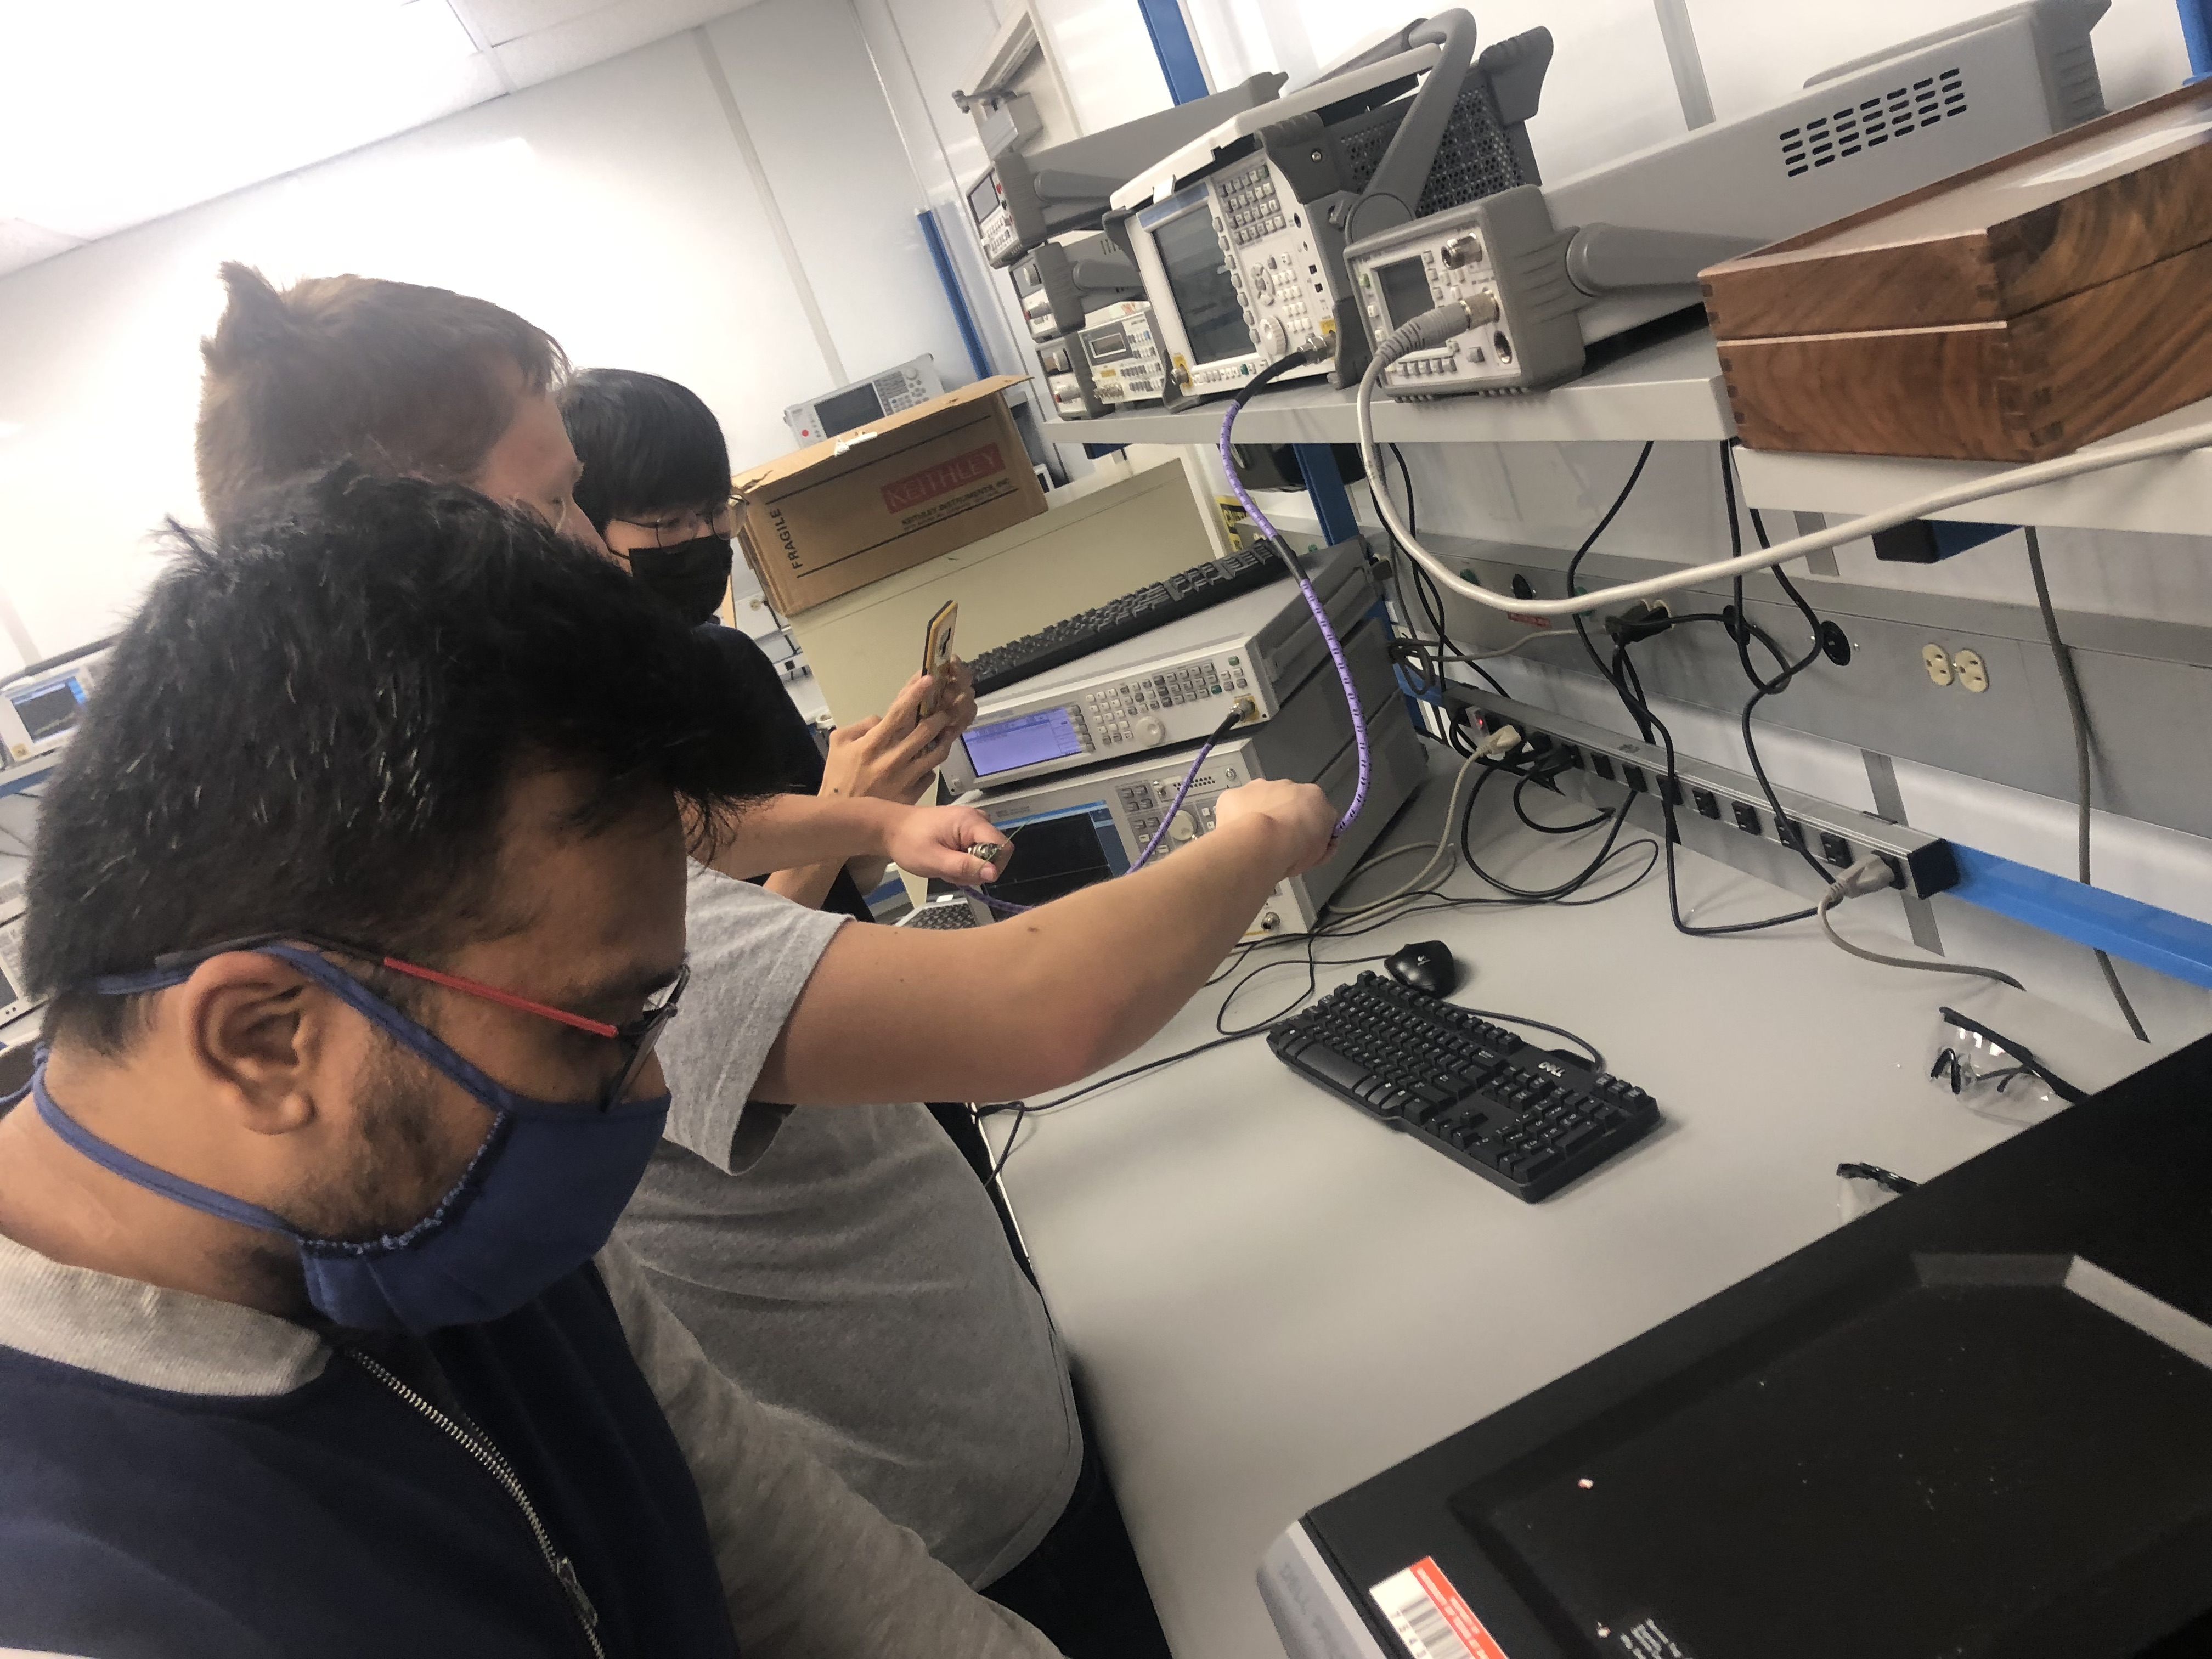
\includegraphics[width=0.3\textwidth]{txrx_setup.jpg}
    \caption{\label{fig:txrx_setup} Antenna to Antenna Power Measurement Setup}
\end{figure}


\section{Discussion and Summary}

Overall, in this lab familiarity with antennas and cell phone operation was
gained. The importance of antennas in modern society was realized. Significant
design decisions such as length of the antenna wires and orientation of
communicating antennas showed the nuance behind wireless communication.
\appendices
\section{Pre-Lab}
\textbf{Design a half-wave dipole antenna using wire and an RF SMA connector.
    The wire and the RF connector will be provided in the lab.}

In the prelab, it was estimated the the operating frequency was 850 MHz.
\begin{align*}
    c                  & =\lambda f                               \\
    \lambda            & =\frac{c}{f}                             \\
    \lambda            & =\frac{3\times 10^{8}}{850\times 10^{6}} \\
    \lambda            & =0.352941\text{m}                        \\
    \lambda            & =35.2941\text{cm}                        \\
    \frac{\lambda }{2} & =17.6471\text{cm}                        \\
    \frac{\lambda }{4} & =8.82353\text{cm}
\end{align*}

% \section{Extra Photos}

\end{document}